\documentclass[11  pt]{article} 
\usepackage[lmargin=1in,rmargin=1.75in,bmargin=1in,tmargin=1in]{geometry}  


% For hyperlinking everything
\usepackage{hyperref}
\hypersetup{
	colorlinks=true, %set true if you want colored links
	linktoc=all,     %set to all if you want both sections and subsections linked
	linkcolor=blue,  %choose some color if you want links to stand out
}


\usepackage[latin1]{inputenc}
\usepackage{amsmath}
\usepackage{mathrsfs}  
\usepackage{amsfonts}
\usepackage{amssymb}
\usepackage{graphicx}
\usepackage{subfig}
\usepackage{caption}
\usepackage{algorithm}
%\usepackage{algcompatible}
%\usepackage{algorithmicx}
\usepackage{algpseudocode}

\usepackage{titlesec}
\titleformat{\section}{\fontfamily{lmss}\fontsize{14}{15}\bfseries}{\thesection}{1em}{}
\titleformat{\subsection}{\fontfamily{lmss}\fontsize{12}{15}\bfseries}{\thesubsection}{1em}{}




\usepackage{amsthm}

\newtheoremstyle{noit}
{10pt}% <Space above>
{10pt}% <Space below>
{}% <Body font>
{}% <Indent amount>
{\bfseries}% <Theorem head font>
{.}% <Punctuation after theorem head>
{.5em}% <Space after theorem headi>
{}% <Theorem head spec (can be left empty, meaning `normal')>

\newtheoremstyle{example}
{10pt}% <Space above>
{10pt}% <Space below>
{}% <Body font>
{20pt}% <Indent amount>
{\bfseries}% <Theorem head font>
{.}% <Punctuation after theorem head>
{.5em}% <Space after theorem headi>
{}% <Theorem head spec (can be left empty, meaning `normal')>


\newtheoremstyle{indented}{20pt}{20pt}{\addtolength{\leftskip}{2.5em}}{}{\bfseries}{.}{.5em}{}


\newtheorem{theorem}{Theorem}
\numberwithin{theorem}{section}
\newtheorem{lemma}[theorem]{Lemma}
\newtheorem{corollary}[theorem]{Corollary}
\newtheorem{observation}{Observation}
%\numberwithin{observation}{section}
%\numberwithin{definition}{section}
\newtheorem{conjecture}{Conjecture}
\newtheorem{Qu}{Question}
\newcommand{\QU}{\begin{Qu}\normalfont}

\theoremstyle{noit}
\newtheorem{fact}{Fact}
\newtheorem{definition}{Definition}

\theoremstyle{indented}
\newtheorem{example}{Example}

\theoremstyle{indented}
\newtheorem{problem}{Problem}


%\newenvironment{proof}{\noindent{\bf Proof:} \hspace*{1em}}{
%    \hspace*{\fill} $\Box$ }
%\newenvironment{proof_of}[1]{\noindent {\bf Proof of #1:}
%    \hspace*{1em} }{\hspace*{\fill} $\Box$ }
%\newenvironment{proof_claim}{\begin{quotation} \noindent}{
%    \hspace*{\fill} $\diamond$ \end{quotation}}
\newcommand{\vs}[1]{\vspace{#1}}

\newcommand{\lecture}[2]{
 \noindent
\begin{center}
	\framebox{
		\vbox{
			\hbox to 5.78in { {\bf CSCE 411: Design and Analysis of Algorithms} \hfill  }
			\vspace{2mm}
			\hbox to 5.78in { {\Large \hfill Lecture #1\hfill} }
			\vspace{2mm}
			\hbox to 5.78in { {\it Date: #2 \hfill Lecturer: Nate Veldt} }
		}
	}
\end{center}
\vspace*{4mm}
}


\newcommand{\hw}[2]{
	\noindent
	\begin{center}
		\framebox{
			\vbox{
				\hbox to 5.78in { {\bf CSCE 411: Design and Analysis of Algorithms} \hfill  }
				\vspace{2mm}
				\hbox to 5.78in { {\Large \hfill Homework #1\hfill} }
				\vspace{2mm}
				\hbox to 5.78in { {\it Due date: #2 \hfil} }
			}
		}
	\end{center}
	\vspace*{4mm}
}



\newcommand{\under}[1]{\underline{\hspace{#1}}}
\setlength{\parindent}{0em}

%\usepackage[tagged]{accessibility}

% Graph terms
\newcommand{\vol}{\textbf{vol}}
\newcommand{\cut}{\textbf{cut}}


% Matrices
\newcommand{\mA}{\textbf{A}}
\newcommand{\mB}{\textbf{B}}

% vectors
\newcommand{\ve}{\textbf{e}}
\newcommand{\vx}{\textbf{x}}


% Other
\newcommand{\calN}{\mathcal{N}}

\usepackage{mathtools}
\DeclarePairedDelimiter\ceil{\lceil}{\rceil}
\DeclarePairedDelimiter\floor{\lfloor}{\rfloor}


\newcommand*{\aitem}{ \item[{
\includegraphics[width=0.8cm,height=0.5cm]{../../Lectures/figures/A}} ]  }
\newcommand*{\bitem}{ \item[{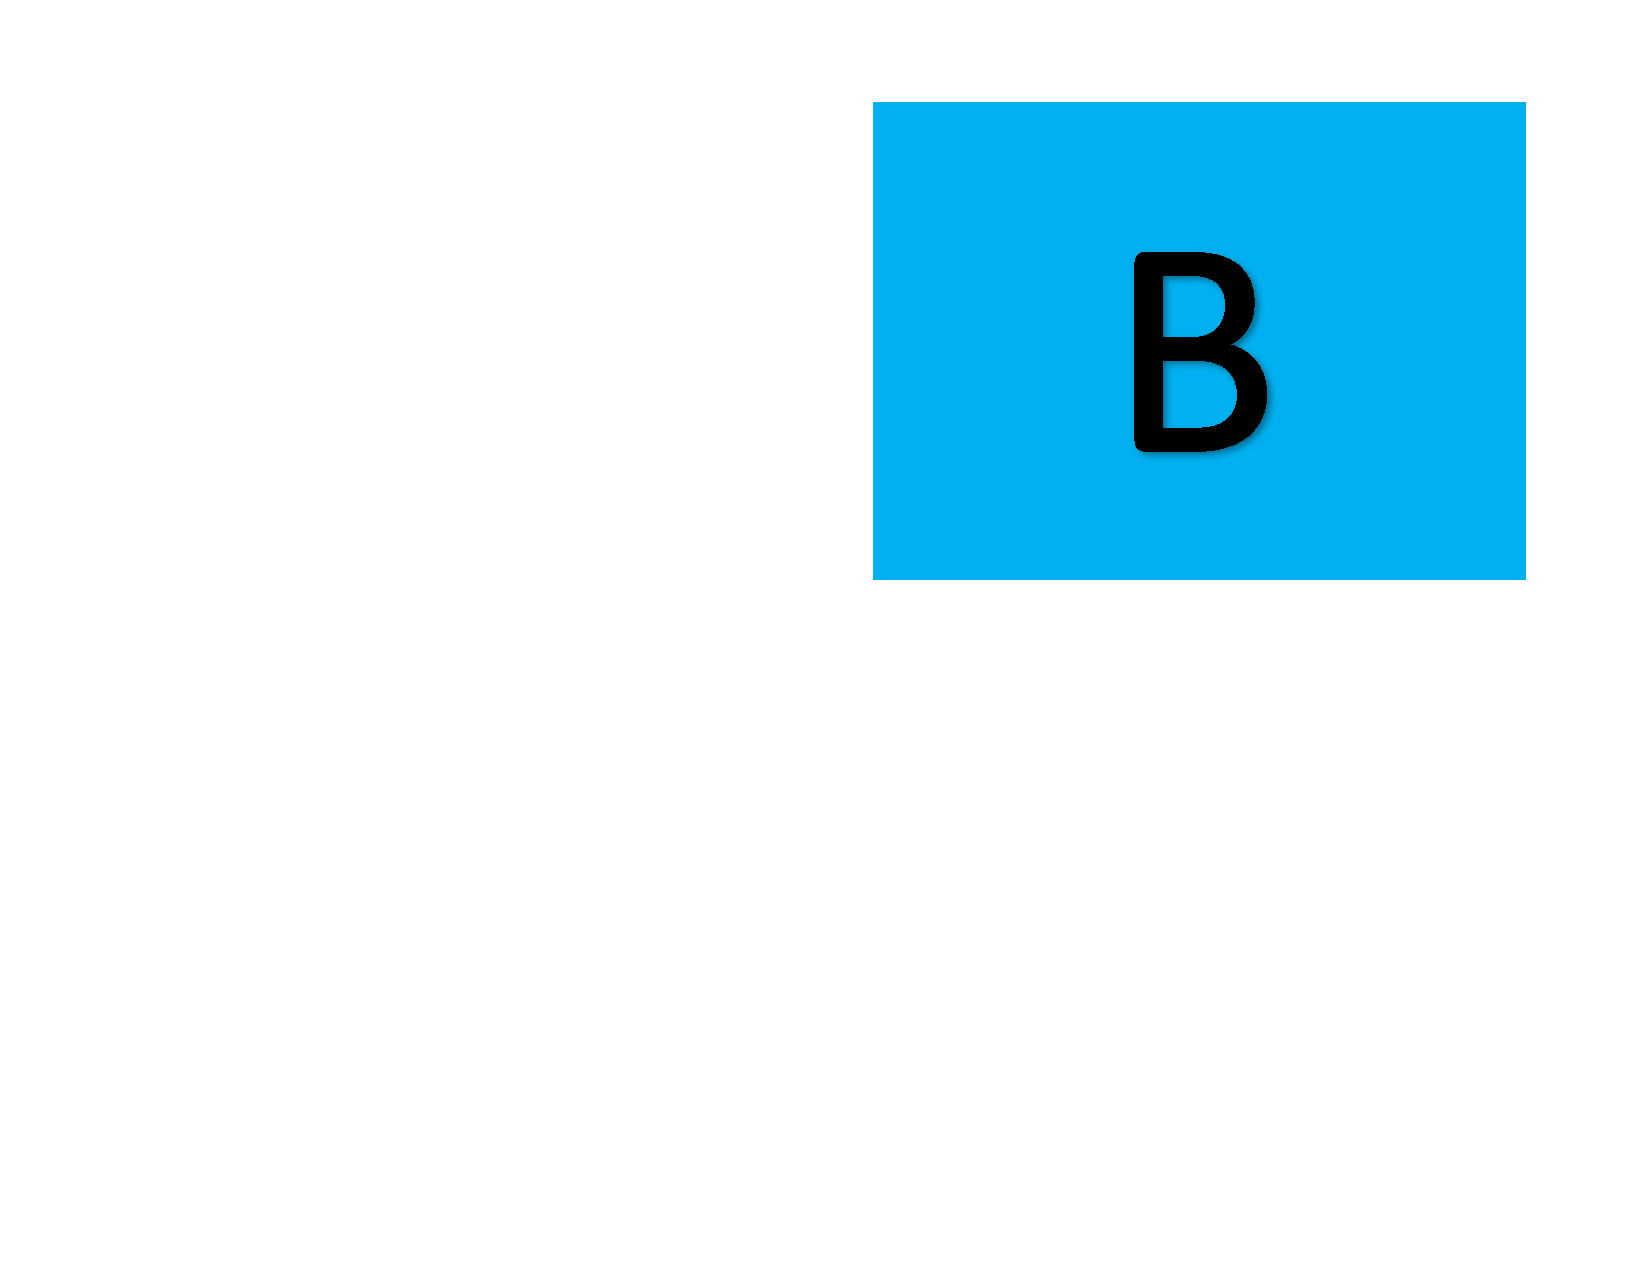
\includegraphics[width=0.8cm,height=0.5cm]{../../Lectures/figures/B}} ]  }
\newcommand*{\citem}{ \item[{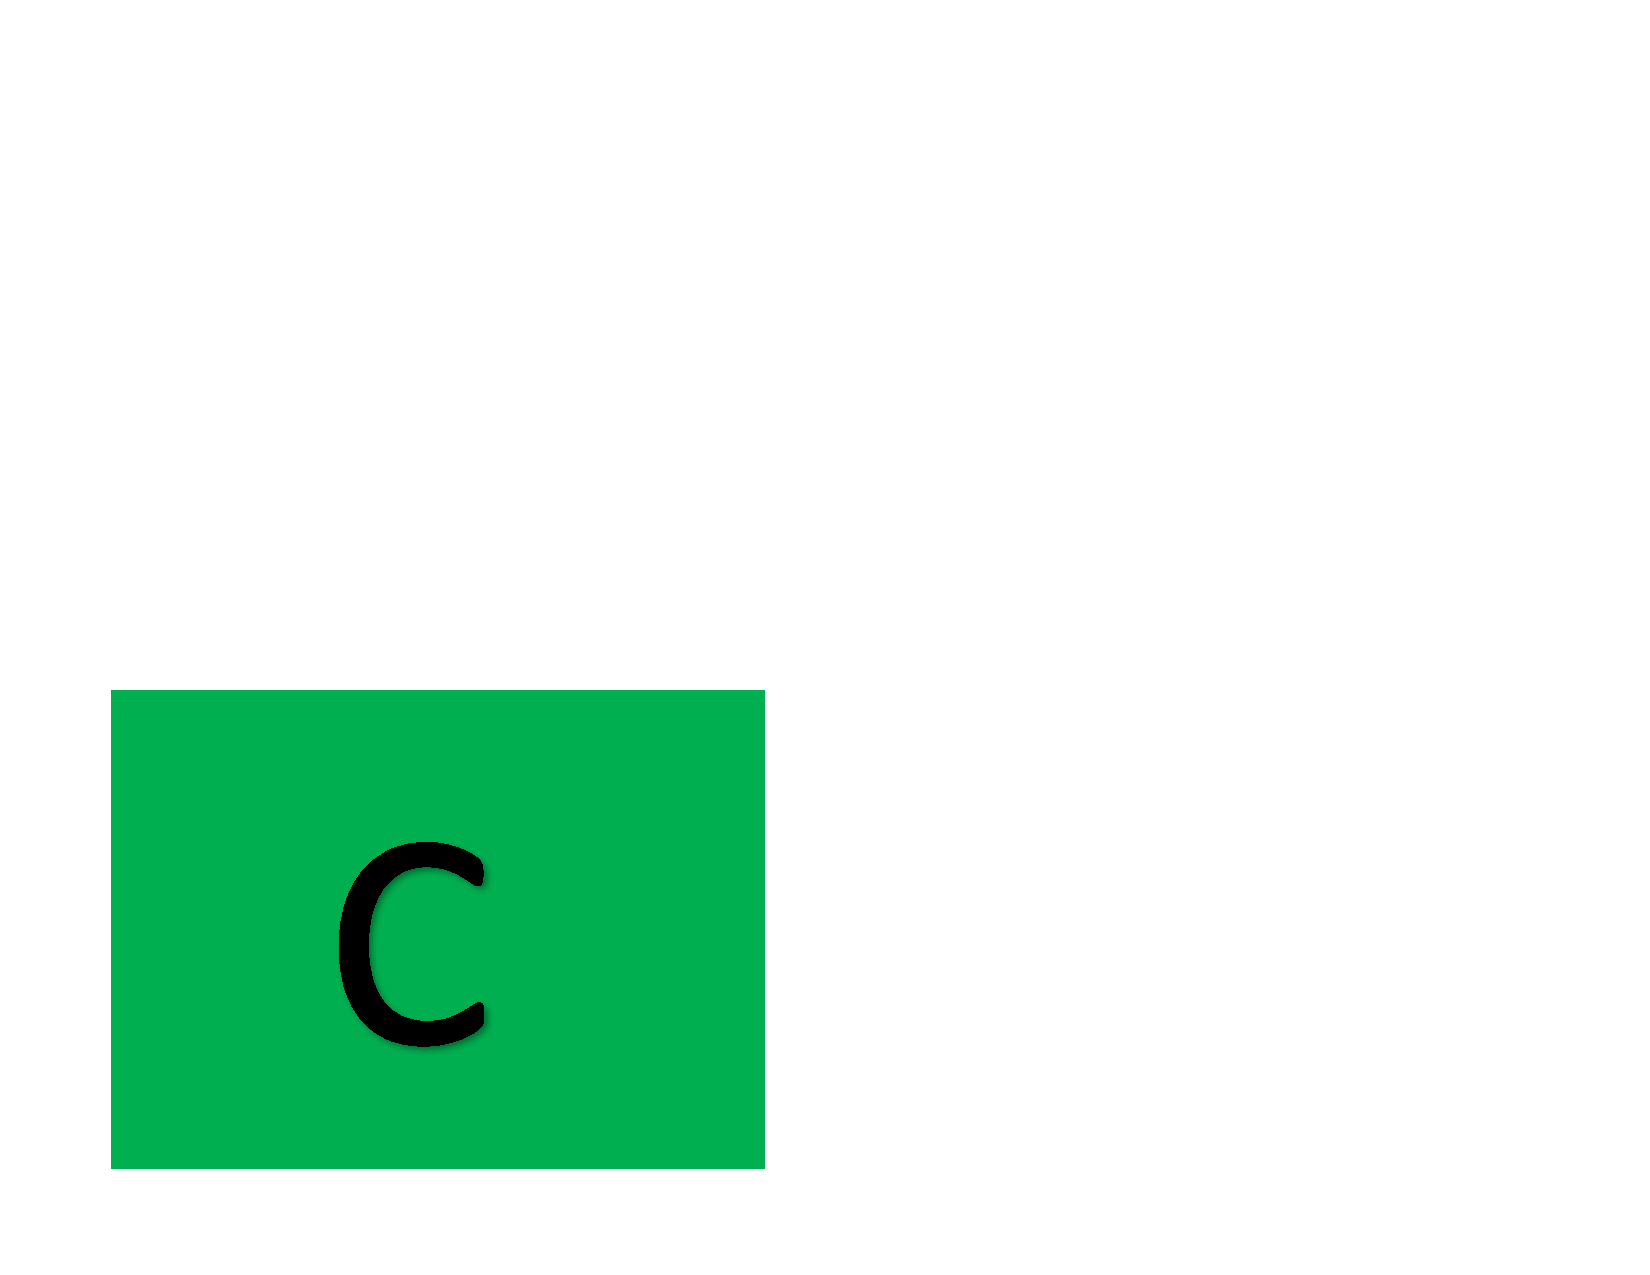
\includegraphics[width=0.8cm,height=0.5cm]{../../Lectures/figures/C}} ]  }
\newcommand*{\ditem}{ \item[{
\includegraphics[width=0.8cm,height=0.5cm]{../../Lectures/figures/D}} ]  }
\newcommand*{\eitem}{ \item[{
\includegraphics[width=0.8cm,height=0.5cm]{../../Lectures/figures/E}} ]  }
\newcommand*{\fitem}{ \item[{
\includegraphics[width=0.8cm,height=0.5cm]{../../Lectures/figures/F}} ]  }


\newcommand{\hide}[1]{\underline{\phantom{#1 #1}}}

\usepackage{setspace}

\onehalfspacing

\begin{document}
	
	\lecture{19: Computational Complexity: P and NP}{April 8}
	
	\section{The universe of computational problems}
	\vspace{5cm}
	

	
	\paragraph{Refresher on computational problems}
	It will be important for us to distinguish between three concepts in defining and solving computational problems:
	\begin{enumerate}
		\item Problem: a computational task that takes in an input and seeks a specific output. \\ \\
		\item Instance:  one specific input for the problem \\ \\
		\item Candidate solution: the data encoding a possible solution to an instance. \\ \\
	\end{enumerate}

	\newpage
	
	\subsection{Decision Problems and Optimization Problems}
	A computational problem $Q$ is a \emph{decision} problem if \\%it has a YES or NO solution for any input $i$. \\
	
	
	\vfill
	
	An optimization problem is a problem that seeks the minimum or maximum value of a function subject to constraints. \\
	
		\begin{Qu}
		Which of the following is a decision problem?
		\begin{itemize}
			\aitem Find the maximum flow for a graph $G = (V,E)$ with source/sink nodes $s$ and $t$.
			\bitem Find if the graph $G = (V,E)$ is connected.
			\citem Find the shortest path of a graph $G = (V,E)$
			\ditem Find if $G = (V,E)$ is a directed acyclic graph
			\eitem More than one of the above
		\end{itemize}
	\end{Qu}

	
		For any optimization problem, we can define a corresponding \emph{decision} problem by taking an extra input $k$ and asking:
	
%	\begin{center}
%		Does there exist a solution with value less than $k$ (or $> k$ for maximization problems).
%	\end{center}
	\vfill

	\newpage

	\subsection{The problem class $P$}
	A problem $Q$ is said to be in $P$ if there is a polynomial time algorithm that solves the problem. \\
	
	
	In other words, if $n$ is the size of the input data, the problem has a runtime such as: \\ \\
	
		\vs{2cm}
		
	These are often referred to as \hide{tractable} problems and are treated in theory as problems that can be solved \hide{quickly}. \\
	
	\vs{10cm}
	
	All of the problems we have considered so far are polynomial time, but this is only a small sample of problems. \\
	
	
	\newpage
	\subsection{The problem class NP}
	We'll define NP problems using a few different levels of technical difficulty.
	
	\paragraph{Level 1: informal, gets us most of the way there.}
	A problem is in NP if we can check in polynomial time whether a given candidate solution solves the instance or not.\\
	
	
	
	
	\vs{6cm}
	
	\paragraph{Level 2: certificates and verifiers.}
	NP is the set of decision problems with the following property: \\
	
	If the answer to an instance is \emph{yes}, there exists some data called a \emph{certificate} with which an algorithm can \emph{verify} the answer is YES in polynomial time. \\
	
	The \emph{certificate} is \\%the YES solution. \\
	
	
	The \emph{verifier} is  \\ %the algorithm that confirms the solution is YES by checking. \\
	
	
	\newpage
	\paragraph{Level 3: the technically precise definition.}
	NP is the set of decision problems that can be solved by 
	%a \textit{nondeterministic Turning machine} in polynomial time. \\
	
		\vs{2cm}
		
	This involves defining Turing machines, formal languages, and a whole lot more.

	\vs{2cm}
	
	You do not need to process this definition (or all the textbook details) for this course. But it does tell us where the name ``NP'' comes from:\\
	
	%NP means ``Nondeterministic Polynomial'' time. \\
	
	
	\newpage
	
	\paragraph{Examples}
	A problem is in NP if for every YES instance there is a \emph{certificate} that an algorithm can use to \emph{verify} in polynomial time that it is truly a YES instance. \\
	
	\textbf{Example 1.} Does $G = (V,E)$ have a clique of size at least $k$? \\
	
	\textbf{Certificate} \\%A set of $k$ nodes that is a clique. \\
	
	
	\textbf{Verifier} \\ %Check each pair of nodes and make sure they all have an edge between them. \\ \\
	
	\vfill
	\textbf{Example 2.} Is $G = (V,E)$ a connected graph? \\
	
	\textbf{Certificate} \\ \\ %The entire graph $G$. \\
	
	
	\textbf{Verifier} \\ \\ %Run a BFS on $G$ an \\ \\
	
	\vfill
	
	\noindent \textbf{Proving something is in NP:}
	\emph{If you can check in polynomial time whether a candidate solution solves the problem or not, then the problem is in NP.}
	
	\newpage 
	
%	\paragraph{Other examples (practice)}
%	Consider the following definitions for an unweighted and undirected graph $G = (V,E)$.
%	\begin{itemize}
%		\item A simple path is a path in $G = (V,E)$ that contains no cycles
%		\item A clique is a set of nodes $S$ where every pair of nodes in $S$ defines an edge.
%		\item A Hamiltonian cycle is a path of edges in a graph $G = (V,E)$ that goes through each node exactly once.
%	\end{itemize}
%	
%	\vs{2cm}
%	
%	
%	For the following problems, discuss and answer whether they are in NP. What is the certificate and verifier if it is in NP? Can you prove if any of them are in P? 
%	\begin{itemize}
%		\item Find whether the graph $G = (V,E)$ contains a clique with $k$ nodes or more.
%		\item Find whether the graph $G = (V,E)$ is connected.
%		\item Find whether $G = (V,E)$ has a Hamiltonian cycle.
%		\item Find whether the shortest simple path in $G$ has less than or equal to $k$ edges.
%		\item Find whether the graph contains a cycle.
%		\item Find whether the longest simple path in $G$ has greater than or equal to $k$ edges.
%	\end{itemize}
%	
%	\newpage
	\subsection{The co-NP class}
A problem is in co-NP if for every \hide{NO instance } there is a \emph{certificate} (some data) that an algorithm can use to \emph{verify} in polynomial time that it is truly a \hide{ NO instance.} \\ \\

To be clear, we will often use the terms \hide{NO}-certificate and \hide{NO}-verifier. \\ \\


\textbf{Example problem} Is $G = (V,E)$ a directed acyclic graph? \\ \\

\vs{2cm}

\textbf{Certificate} \\ \\ %A set of nodes that defines a cycle. \\ \\

\vs{2cm}

\textbf{Verifier} \\ \\ %Check that the set of nodes is a cycle. \\ \\


\vfill

\textbf{Conclusion}: Checking whether $G$ is a DAG is \hide{in co-NP. }  \\
\vs{1cm}

\newpage

\begin{Qu}
	The verifier we showed for the clique problem will return YES if the $k$ nodes are a clique, and will return NO if the $k$ nodes are not a clique. \\
	
	True or false: this means that this algorithm is also a NO-verifier, and so the clique problem is also in co-NP.
	\begin{itemize}
		\aitem True
		\bitem False
	\end{itemize}
	
	
\end{Qu}

\vfill

\begin{Qu}
	Checking whether $G$ is a DAG in in co-NP. Is it also in NP? 
	\begin{itemize}
		\aitem Yes
		\bitem No
	\end{itemize}
	
\end{Qu}
\vfill
\newpage
\section{Reductions}
A reduction is a mapping from one computational problem to another.  \\ 

\textbf{Definition} Let $A$ and $B$ be decision problems. We say that $A$ can be reduced to $B$ if

\begin{itemize}
	\item For every instance of $A$ we can define a corresponding instance of $B$ such that
	\item All YES instances in $A$ map to YES instances in $B$
	\item All NO instances in $A$ map to NO instances in $B$
\end{itemize}

\vfill

This is a polynomial-time reduction if this conversion process takes polynomial time. \\

This seems obvious: what's an example of a reduction that is not polynomial-time? \\ \\

\vfill

\newpage
\subsection{Reduction and complexity}

If $A$ can be reduced to $B$ in polynomial time, we denote this by 

\begin{equation*}
	\hide{A \leq_p B}
\end{equation*}

This implies that:
\begin{itemize}
	\item $A$ is easier\footnote{where easier might mean ``no harder than''} than $B$, or equivalently 
	\item $B$ is at least as hard as $A$ is to solve\\
\end{itemize} 

\begin{lemma} 
	If $B \in P$ and \hide{$A \leq_p B$}, then \hide{ $A \in P$.}
\end{lemma}	

\newpage


\section{NP-completeness}

\textbf{Definition: } A problem $Q$ is NP-complete if:
\begin{enumerate}
	\item $Q \in$ NP
	\item for every problem $B \in \text{NP}$, $B \leq_p Q$. \\
\end{enumerate}

\textbf{In words:} \\ %a problem is NP-complete if it is NP and you can reduce any problem in NP to it. \\


\vs{8cm}

This implies that NP-complete problems are the \emph{hardest} problems in NP. \\


Why? Remember that $A \leq_p B$ means $A$ is easier than $B$. \\

In fact, if you only take the second part of the definition, this defines the set of NP-hard problems.



%\newpage
%
%\section{Views of the computational problem universe}
%There are four different possibilities for the relationship between P, NP, and co-NP.
%
%
%
%\vfill
%
%There are two possibilities for the relationship between P, NP, and NP-complete.
%
%\vfill
%
%\newpage
%
%\paragraph{A few famous NP-complete problems}
%\begin{itemize}
%	\item Find if a graph has a clique of size at least $k$
%	\item Find if a graph has a Hamiltonian cycle
%	\item Find if a graph has a simple path with at least $k$ edges
%	\item \textbf{Subset sum}: given a set of numbers, find if any subset sums to zero
%	\item \textbf{SAT}: Logic problems we will look at in more depth later
%\end{itemize}


	

	
	
\end{document}